\section{Identification of metal foils by their absorption edges}
\label{sec:absorb}

In the following section, we are going to identify an unknown metal foil due to its absorption edges. The used setup is described in section (ref).
The setup is able to measure the transmitted intensity in regards to a diffraction angle. The measured angle $\omega$ (=$2\Theta$) can be varied from 
5.0° $\leqslant \, \omega \, \leqslant$ 51.0° with a step width of 0.1°. In the beam path, we placed two foils marked with an index $N$ of thickness $d = \SI{2.5e-3}{cm}$. In the following, they shall be called \textit{F11} and \textit{F8} for foil 11 and 8.
The thickness $d$ is treated as if it has no deviation. As in spectroscopy, a reference measurement is performed. In the 
second measurement, one foil at a time is put in place and the measurement is repeated. 

\subsection{Calibration of the device}

Since we are not sure if the calibration of the equipment is correct, we perform our own calibration.
For this we use the well know characteristic radiation of our Tungsten anode. The sharp peaks should be visible in the 
intensity spectrum if they fulfill the Bragg condition

\begin{equation}
    2 d \sin{\omega} = n \lambda
\end{equation}

with $\omega$ being same angle mentioned above, $ \lambda $ being the wavelength of the spectrum and $d$ being the grid plane spacing. The cubic $\mathrm{CaF}_2$ crystal has a 
grid plane distance 

\begin{equation}
    d_{hkl} = \sqrt{\frac{a^2}{h^2+k^2+l^2}}
\end{equation}

with $(hkl) = (220) $ being the Laue indexes and $a = \SI{5.463 \pm 0.001 }{ \angstrom}$. Therefore, $d = \SI{1.9314 \pm 0.0004}{ \angstrom} $ in this geometry.

Assuming the dominant peaks for lower angle are peaks due to the first order of the diffraction, we correlate those with the well know peaks from literature. The tabulated values for the characteristic peaks of the wolfram anode are from \textit{National Institute of Standards and Technology} (see ref).
Transforming the peak values given in $\lambda$ into angles in our geometry and taking into account their relative intensity, the peaks are identifiable.
The observed peaks are the peaks from the \textit{Lyman series} as shown in Figure (fig).
\begin{figure}
    \centering
    \begin{subfigure}[b]{0.85\textwidth}
        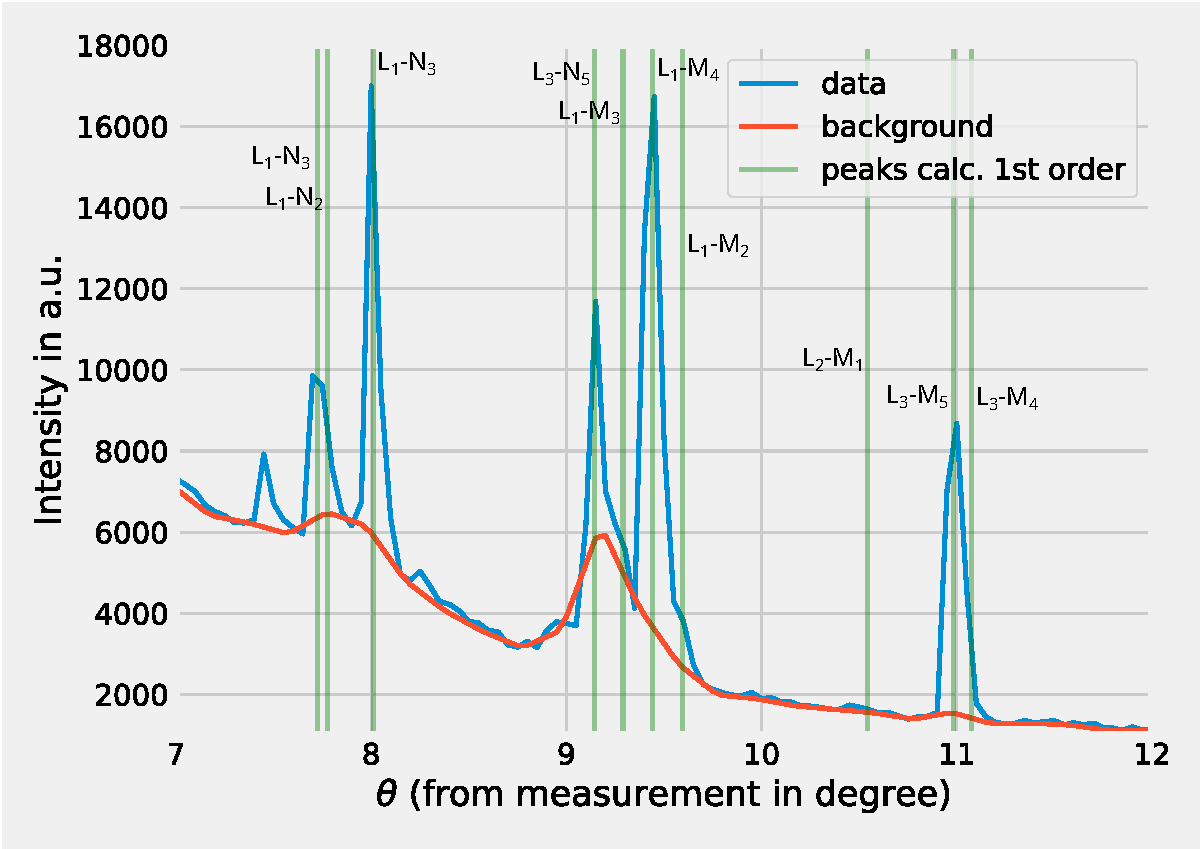
\includegraphics[width =\textwidth]{Programming/Absorption/MatchLine1Edit.pdf}      
        \caption{Matching the first-order diffraction peaks of the tungsten X-ray tube}
      \label{fig:MatchLine1}
    \end{subfigure}
    \vspace{0.3cm}

    \begin{subfigure}[b]{0.85\textwidth}
      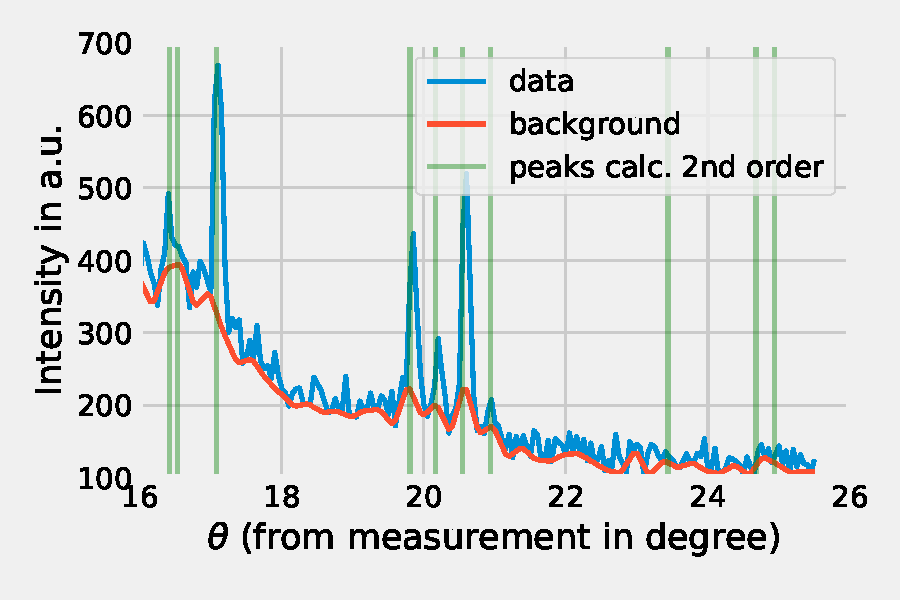
\includegraphics[width = \textwidth]{Programming/Absorption/MatchLine2.pdf}      
      \caption{Matching the second-order diffraction peaks of the tungsten X-ray tube}
      \label{fig:MatchLine2}
    \end{subfigure}
    \caption{The peaks in the intensity of the X ray device are matched with the tabulated characteristic radiation peaks. The green lines are the angles at which the characteristic radiation of the tungsten X-ray anode should appear. In (a) the peaks are named with the IUPAC nomenclature.}
    \label{fig:Peaks}
\end{figure}

\begin{figure}[h!]
    \centering
    \begin{subfigure}[b]{0.48\textwidth}
        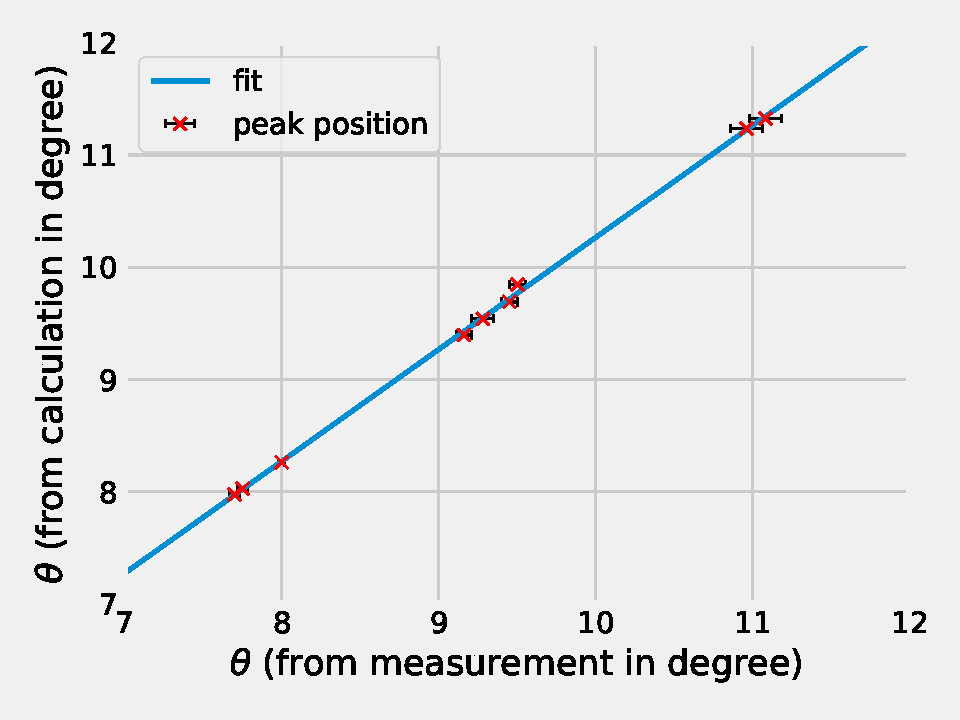
\includegraphics[width =\textwidth]{Programming/Absorption/Eichung1ref.pdf}      
        \caption{Fit for the first-order diffraction}
      \label{fig:subfig1}
    \end{subfigure}
    \hfill
    \begin{subfigure}[b]{0.48\textwidth}
      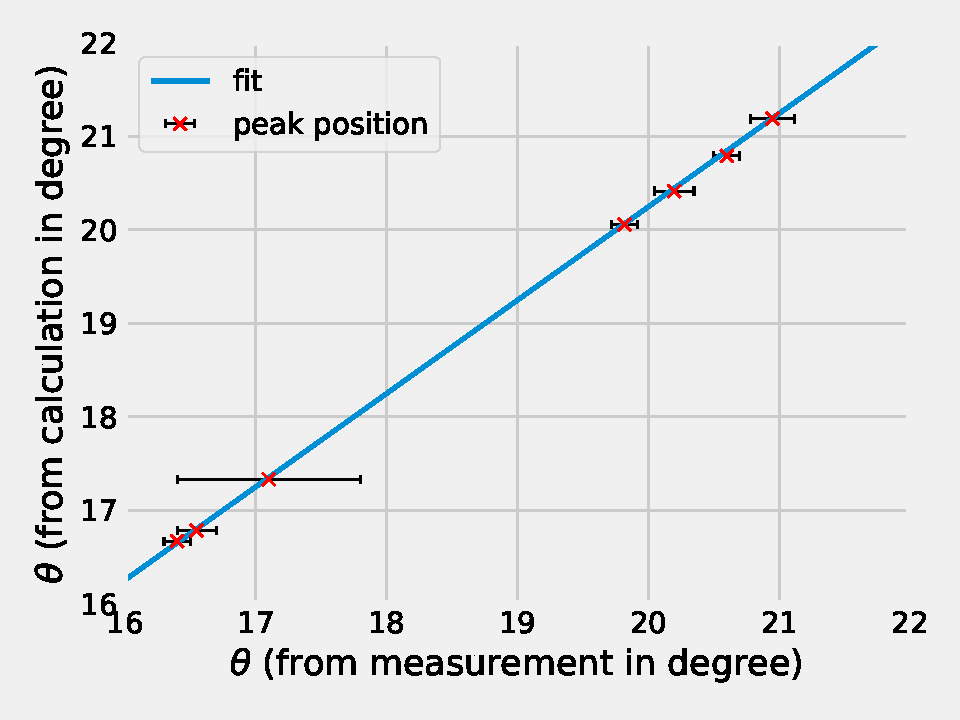
\includegraphics[width = \textwidth]{Programming/Absorption/Eichung2ref.pdf}  
      \caption{Fit for the second order reflection}
      \label{fig:subfig2}
    \end{subfigure}
    \caption{The extracted peaks are compared to the tabulated values and are fitted with a line of the form $y = m\cdot x + t$.}
    \label{fig:mainfig}
\end{figure}

To calibrate our device, we assume the the scale is linear and has to parameters to vary: an offset $t$ and the slope $m$. Therefore, we 
fit a straight line to our data plotted against the theoretical value. As can be seen in Figure (Fig.), the assumption of a linear process is well founded. 
These two parameters will be used to calibrate our device from now on. Before continuing, we have to verify the aforementioned presupposition that we are observing the first diffraction order.
Thus, we investigate the spectral range where we would expect the second order of peaks to appear and as show in Figure (fig) we find the expected peaks -- which are also in accordance with the calibration made before.


\subsection{Identifying metals due to their absorption edges}

As we plot the spectra against the wavelength or energy, we can see distinct absorption edges. Before analyzing those, 
we want to draw the readers attention to a commonly made mistake when changing the x-scale of intensity spectra.

It is \textbf{not} sufficient to simply rescale the axis to a different quantity, as the relation
\begin{equation*}
    I(\theta) \mathrm{d}\theta = I(\lambda) \mathrm{d}\lambda
\end{equation*}
has to be fulfilled. Reformulating this in our context using the Bragg equation , we reach the relation 
\begin{equation}
    \frac{I(\lambda)}{I(\theta)} = \frac{d \lambda}{d \theta} = \frac{2 d \cos(\theta)}{m}.
\end{equation}
This tells us how to rescale the intensity spectrum when changing the dependencies, in this case 
\begin{equation}
    I(\lambda) = I(\theta) \cdot  \frac{d \lambda}{d \theta} = I(\theta) \cdot \frac{2 d \cos(\theta)}{m} .
\end{equation}

When a metal is irradiated with X-rays, strong, irregular absorption bands become visible. These are created when the electrons exceed a certain energy form, they can interact and
free electrons from lower energy levels of the atom.  This leads to a sharp jump in the absorption.
This quantity
\begin{equation}
    \frac{\mu}{\rho} = \frac{1}{\rho x}\log(\frac{I_0}{I})
\end{equation}

is derived from the Beer-Lamber law.
\begin{figure}[ht]
    \centering
    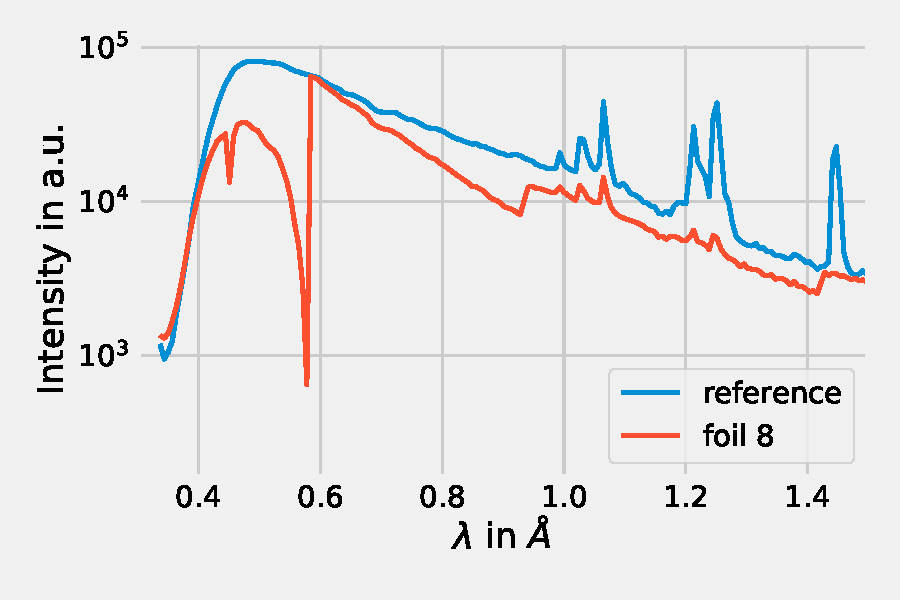
\includegraphics[width = 0.75\textwidth]{Programming/Absorption/absorptionskanteFit.pdf}
    \caption[short]{X-ray intensity spectrum  of foil 8 plotted against the reference signal. The absorption edge in F8 are well visible.}
    \label{fig:IntF8ref}
\end{figure}
The specific energy at which those jumps take place depend on the internal energetically structure of 
the atom, especially on the number of protons. Therefore, it is possible to distinguish the different metals. For \textit{F8} as shown in \ref{fig:IntF8ref}, we observe the absorption band at 
\SI{0.58\pm0.01}{ \angstrom}, which is very close to the wavelength of the K absorption edge of Technetium (Tc), whereas foil 11 has a K edge close to Molybdenum (Mo) and one close to Palladium (Pd). For \textit{F11} we are not sure whether a
measurement error occurred here, since the absorption does not have the shape we expected. In \textit{F11}'s absorption spectrum, we see two absorption edges to close to be a K edge and L edge. Therefore we expect the foil to consist of two metals.

We can not observe the second order diffraction from the absorption edges. The other edges we observe in Figure \ref{fig:F8edge} are also not the further K transitions of Molybdenum. The L edges are far off at about 5 \AA. This spectral range could be observed with this setup by changing the voltage on the X-ray device. Therefore, we can not identify the edges in this spectrum. 

\begin{figure}[h]
    \centering
    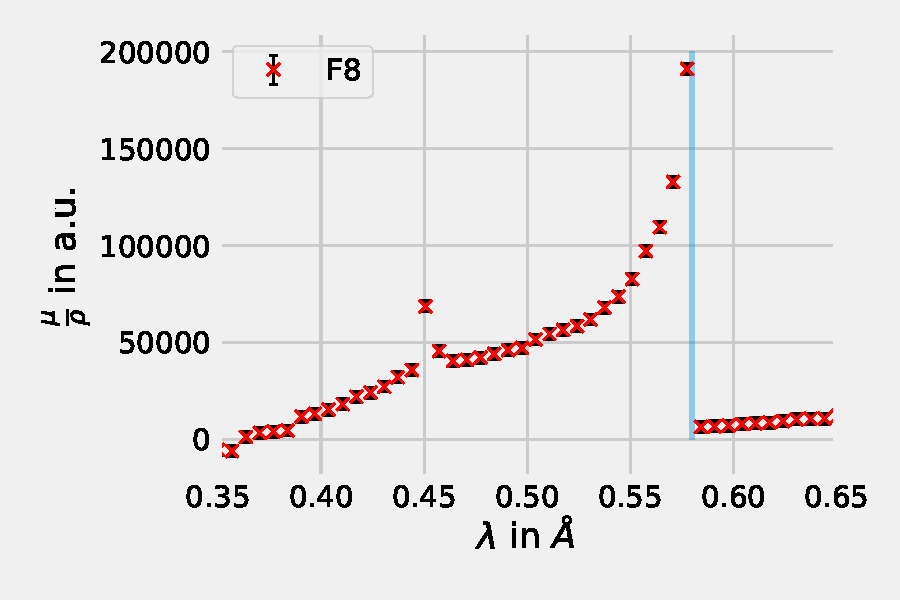
\includegraphics[width = 12cm]{Programming/Absorption/F8Kedge.pdf}
    \caption{The absorption takes a sharp jump for the foil 8 close to $\lambda$ = \SI{0.58\pm0.01}{\angstrom}. The errors are calculated from the  relative fluctuations far away from the any peaks. Those are takes as the relative intensity error. It is assumed that the thickness has no deviation.}
    \label{fig:F8edge}
\end{figure}


\begin{figure}[ht]
    \centering
    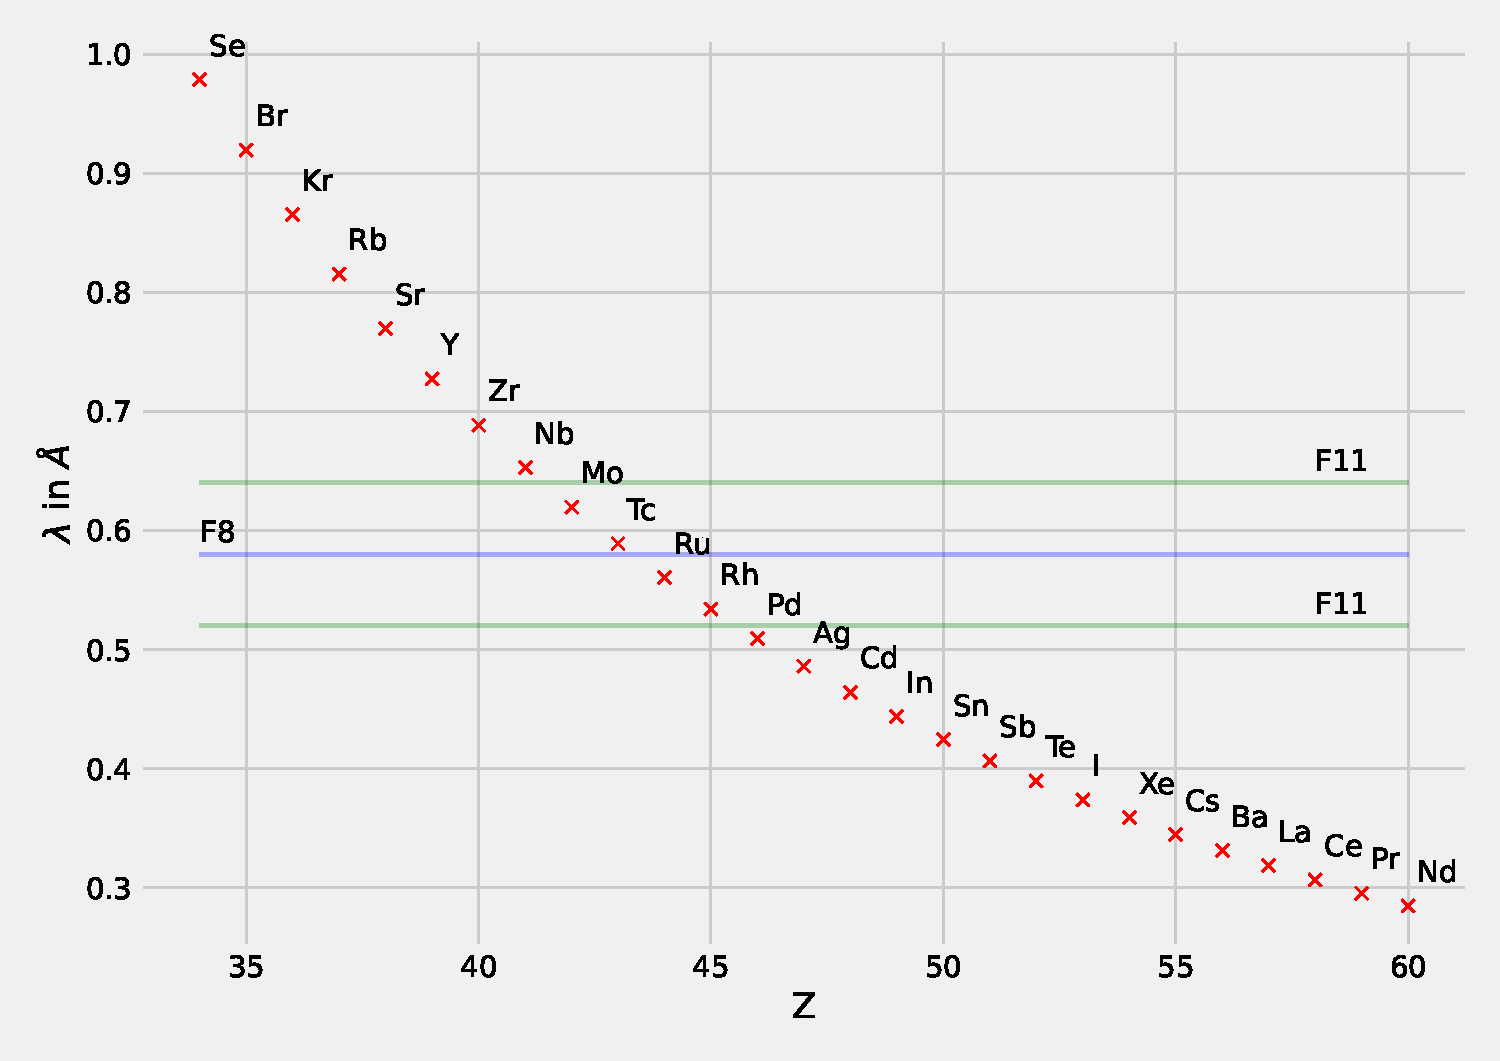
\includegraphics[angle = 90, width = 0.95\linewidth]{Programming/Absorption/Elements.pdf}
    \label{fig:Elements}
    \caption{Wavelength of the K-edge for different elements with increasing ordinal number. From (ref)}
\end{figure}


\begin{table}[ht]
    \centering
    \begin{tabular}{lrr}
        \toprule
        transition & eneryineV & EdgeInA \\
        \midrule
        KL1 & 17135.00 & 0.72 \\
        KL3 & 17479.10 & 0.71 \\
        KM1 & 19495.80 & 0.64 \\
        KM3 & 19607.10 & 0.63 \\
        KM4 & 19768.70 & 0.63 \\
        KM5 & 19772.81 & 0.63 \\
        KN1 & 19940.30 & 0.62 \\
        KN3 & 19967.16 & 0.62 \\
        KN4 & 20000.73 & 0.62 \\
        KN5 & 19999.84 & 0.62 \\
        \bottomrule
    \end{tabular}
    \caption{The K transitions of Molybdenum. From }
\end{table}